\begin{figure*}
  \centering
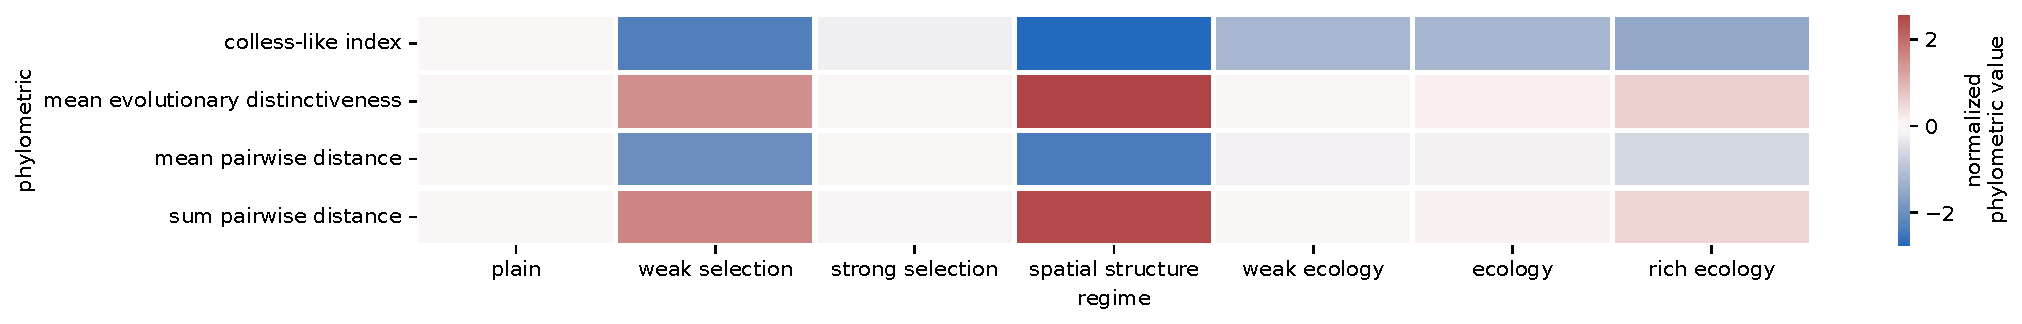
\includegraphics[width=\textwidth]{binder/binder/teeplots/epoch=7+mut_distn=np.random.standard_normal+normed=true+viz=heatmap+x=regime+y=phylometric+ext=.pdf}
\caption{%
  \textbf{Normalized phylometric responses.}
  Heatmap of normalized tree phylometrics across surveyed evolutionary regimes, calculated on perfect-fidelity phylogenies from the simple model.
  Note that normalization shows magnitude of phylometric effect beyond the point of distributional nonoverlap, unlike nonparametric normalization which tops out with complete distributional nonoverlap.
}  
  \label{fig:perfect-tree-phylometrics-heatmap-parametric}
\end{figure*}